\documentclass[11pt]{article}
\usepackage{fullpage}
\usepackage{epsfig}
\usepackage{amsfonts}
\usepackage{amssymb}
\usepackage{amstext}
\usepackage{amsmath}

\begin{document}
\begin{center}
\textbf{Project 2 - Phase 3}\\
\textbf{priyananda ( shenoy@cs.wisc.edu )}\\
\end{center}

1.\\
	X axis points at $(-1,0,0)$ \\
	\[ \left( \begin{array}{cccc}
	-1 & 0    									& 0 					 		& 0 \\
	0  & \frac{-1}{\sqrt{2}} 	& \frac{1}{\sqrt{2}} 	& 0 \\
	0  & \frac{1}{\sqrt{2}}  	& \frac{1}{\sqrt{2}} 	& 0 \\
	0  & 0 											& 0 										& 1 \\
	\end{array} \right) \]
\\
2.\\
	X axis goes to$(-1,0,0)$\\
	Y axis goes to$(0,-\frac{1}{\sqrt{2}},-\frac{1}{\sqrt{2}})$\\
	Z axis goes to$(0,-\frac{1}{\sqrt{2}},\frac{1}{\sqrt{2}})$\\
	
	Matrix form is:
	
	\[ \left( \begin{array}{cccc}
	-1 & 0    & 0 & 0\\
	0  & -\frac{1}{\sqrt{2}} & -\frac{1}{\sqrt{2}} & 0 \\
	0  & -\frac{1}{\sqrt{2}} & \frac{1}{\sqrt{2}} & 0 \\
	0  & 0 & 0 & 1 \\
	\end{array} \right) \]
	
	The inverse matrix is:
	
	\[ \left( \begin{array}{cccc}
	-1 & 0    & 0 & 0\\
	0  & -\frac{1}{\sqrt{2}} & -\frac{1}{\sqrt{2}} & 0 \\
	0  & -\frac{1}{\sqrt{2}}  & \frac{1}{\sqrt{2}} & 0 \\
	0  & 0 & 0 & 1 \\
	\end{array} \right) \]

3. $( \frac{5}{16} , -\frac{3}{16} )$ \\

4.
\begin{figure}[h]
\begin{center}
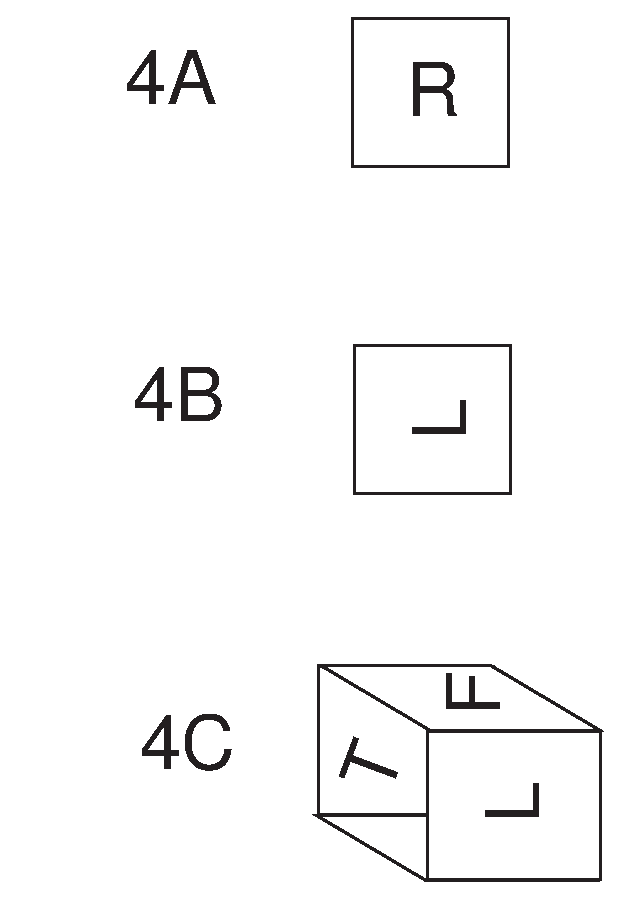
\epsfig{file = hw3.eps, height = 2in, width = 1in}
\end{center}
\end{figure}

5.

	\begin{align*}
	f(u) &= (0,6u) if u \le \frac{1}{6} \\
			 &= (6(u-\frac{1}{6}),1) if \frac{1}{6} \ge u \le \frac{4}{6} \\
			 &= (3,6(u-\frac{4}{6}) + 1 ) otherwise \\
	\end{align*}

6. $f(\frac{1}{2}) = (2, \frac{35}{16})$\\
	 $\acute{f}(\frac{1}{2}) = (5, \frac{-1}{8})$\\
	 $|\acute{f}| = \sqrt{\frac{1601}{8}}$\\

7. $(4, 0), (4, \frac{-8}{3}), (0, -\frac{8}{3}), (0, 0)$\\

8. \\
	First Part: $(0, 0), (0, 1), (\frac{1}{2}, 2), (\frac{5}{4}, \frac{5}{2}), (2, \frac{5}{2})$ \\
	Second Part: $(2, \frac{5}{2}), (\frac{11}{4}, \frac{5}{2}), (\frac{7}{2}, 2), (4, 1), (4, 0)$ 

\end{document}